\chapter{Invariant polynomial functions and covariants}


\section{Polynomial functions}


In this chapter $k$ is an infinite field. We also fix a finite-dimensional $k$-vector space $V$ with basis $(v_1, \ldots, v_n)$.


\begin{defi}
 By $\mc{P}(V)$ we denote set of polynomial functions $V \to k$, i.e. $f \in \mc{P}(V)$ if and only if $f : V \to k$ and there is some $p \in k[X_1, \ldots, X_n]$ such that
 \[
  f\left( \sum_{i=1}^n \lambda_i v_i \right) = p(\lambda_1, \ldots, \lambda_n)
 \]
 for all $\lambda_1, \ldots, \lambda_n \in k$.
\end{defi}


This definition does not depend on the chosen basis. If $(w_1, \ldots, w_n)$ is another basis of $V$ with $w_i = \sum_{j=1}^n a_{ij} v_j$ for $i=1,\ldots,n$ then
\begin{align*}
 f\left( \sum_{i=1}^n \lambda_i w_i \right)
 &= f\left( \sum_{i,j=1}^n \lambda_i a_{ij} v_j \right)
 = p\left( \sum_{i=1}^n \lambda_i a_{i1}, \ldots, \sum_{i=1}^n \lambda_{i} a_{in} \right)\\
 &= p'(\lambda_1, \ldots, \lambda_n)
\end{align*}
for some $p' \in k[X_1, \ldots, X_n]$. So if $f : V \to k$ is a polynomial in $(v_1, \ldots, v_n)$ then also in $(w_1, \ldots, w_n)$.


\begin{rem}
 If a group $G$ acts linearly on $V$ then it acts linearly on $\mc{P}(V)$ by $(g.f)(v) = f\left(g^{-1}.v\right)$.
\end{rem}


\begin{lem}
 There is an isomorphism of rings, even $k$-algebras
 \[
  \mc{P} \xlongrightarrow{\sim} k[X_1, \ldots, X_n]
 \]
 where $n = \dim V$.
\end{lem}
\begin{proof}
 For $1 \leq j \leq n$ define the $j$-th coordinate function (with respect to the chosen basis) as
 \[
  \varphi_j : V \to k, \sum_{i=1}^n \lambda_i v_i \mapsto \lambda_j.
 \]
 By the universal property of the polynomial ring the assignment $X_j \to \varphi_j$ extends to a ring homomorphism
 \[
  \Phi: k[X_1, \ldots, X_n] \to \mc{P}(V), p \mapsto \Phi(p)
 \]
 where
 \[
  \Phi(p)\left(\sum_{i=1}^n \lambda_i v_i\right) = p(\lambda_1, \ldots, \lambda_n).
 \]
 Is it clear that $\Phi$ is surjective. It is left as an exercise to the reader to check that $\Phi$ is injective.
\end{proof}


\begin{lem}\leavevmode
 \begin{enumerate}[a)]
  \item
   Assume $p \in k[X_1, \ldots, X_n]$ with $p(\lambda_1, \ldots, \lambda_n) = 0$ for all $(\lambda_1,\ldots,\lambda_n) \in k^n$. Then $p = 0$.
  \item
   The polynomial functions $\varphi_1, \ldots, \varphi_n \in \mc{P}(V)$ are algebraically independent over $k$, i.e. if $f(\varphi_1, \ldots, \varphi_n) = 0$ for some polynomial $f$ (over $k$) then $f = 0$.
 \end{enumerate}
\end{lem}
\begin{proof}\leavevmode
 \begin{enumerate}[a)]
  \item
   We show this by induction over $n$.
   
   ($n = 1$) Let $p \in k[X_1]$ with $p(\lambda_1) = 0$ for all $\lambda_1 \in k$. Since $k$ is infinite $p$ has infinitely many zeroes. Therefore $p = 0$.
   
   ($n \geq 2$) Assume the claim holds for $n-1$ and $1$. Consider $p \in k[X_1, \ldots, X_n]$ with $p(\lambda_1, \ldots, \lambda_n) = 0$ for all $(\lambda_1, \ldots, \lambda_n) \in k^n$. We write $p$ as
   \[
    p = \sum_{i \in \N} f_i(X_1, \ldots, X_{n-1}) X_n^i
   \]
   with $f_i \in k[X_1, \ldots, X_{n-1}]$ for all $i \in \N$ and $f_i = 0$ for all but finitely many $i \in \N$. Let $(\lambda_1, \ldots, \lambda_{n-1}) \in k^{n-1}$ be fixed but arbitrary. For all $\lambda_n \in k$ we have
   \[
    0 = p(\lambda_1, \ldots, \lambda_n) = \sum_{i \in \N} f_i(\lambda_1, \ldots, \lambda_{n-1}) \lambda_n^i
   \]
   By induction hypothesis we find that $f_i(\lambda_1, \ldots, \lambda_{n-1}) = 0$ for all $i \in \N$. Because $(\lambda_1, \ldots, \lambda_{n-1})$ is fixed but arbitrary we can use the induction hypothesis to get that $f_i = 0$ for all $i \in \N$. So $p = 0$.
  \item
   Assume $f(\varphi_1, \ldots, \varphi_n) = 0$. Then
   \[
    0 = f(\varphi_1, \ldots, \varphi_n)\left(\sum_{i=1}^n \lambda_i v_i\right) = f(\lambda_1, \ldots, \lambda_n)
   \]
   for all $(\lambda_1, \ldots, \lambda_n) \in k^n$. Therefore $f = 0$ by part a). \qedhere
 \end{enumerate}
\end{proof}

\begin{warn}
 The assumption that $k$ is infinite is necessary. If, for example, $p = X^2+X \in \F_2[X]$, then $p(0) = p(1) = 0$, so $p(\lambda)=0$ for all $\lambda \in k$, but $p \neq 0$.
\end{warn}


\begin{cor}
 The map $\Phi : k[X_1, \ldots, X_n] \to \mc{P}(V), X_j \mapsto \varphi_j$ is injective.
\end{cor}


Together with the exercise sheet we find that
\[
 \Phi : k[X_1, \ldots, X_n] \to \mc{P}(V), X_j \to \varphi_j
\]
is an isomorphism of $k$-algebras.


\begin{defi}
 $f \in \mc{P}(V)$ is homogeneous of degree $d \in \Z$ if $f(\lambda y) = \lambda^d f(y)$ for all $\lambda \in k, y \in V$. By definition the zero polynomial $f=0$ is homogeneous of degree $d$ for any $d \in \Z$. For $d \in \Z$ we set
 \[
  \mc{P}(V)_d := \{f \in \mc{P}(V) : f \text{ is homogeneous of degree } d\}.
 \]
\end{defi}


\begin{lem}\leavevmode
 \begin{enumerate}[a)]
  \item
   $\mc{P}(V)_d$ is a $k$-vector space for all $d \in \Z$ (via pointwise addition and scalar multiplication).
  \item
   If $f \in \mc{P}(V)_i$ and $g \in \mc{P}(V)_j$  then $fg \in \mc{P}(V)_{i+j}$, where the multiplication is given by pointwise multiplication.
 \end{enumerate}
\end{lem}
\begin{proof}\leavevmode
 \begin{enumerate}[a)]
  \item For $f_1, f_2 \in \mc{P}(V)_d$ we have
  \begin{align*}
   (f_1+f_2)(\lambda v)
   &= f_1(\lambda v) + f_2(\lambda v)
   = \lambda^d f_1(v) + \lambda^d f_2(v) \\
   &= \lambda^d (f_1(v) + f_2(v))
   = \lambda^d (f_1 + f_2)(v)
  \end{align*}
  for all $\lambda \in k, v \in V$, so $f_1 + f_2 \in \mc{P}(V)_d$. If $f \in \mc{P}(V)$ and $\mu \in k$ then
  \[
   (\mu f)(\lambda v) = \mu f(\lambda v) = \lambda^d \mu f(v) = \lambda^d (\mu f)(v),
  \]
  so $\mu f \in \mc{P}(V)_d$.
  \item
  For all $\lambda \in k$ we have for all $v \in V$
  \[
   fg(\lambda v)
   = f(\lambda v) g(\lambda v)
   = \left(\lambda^i f(v)\right)\left(\lambda^j g(v)\right)
   = \lambda^{i+j} f(v) g(v)
   = \lambda^{i+j} (fg)(v),
  \]
  and therefore $fg \in \mc{P}(V)_{i+j}$. \qedhere
 \end{enumerate}
\end{proof}


\section{Graded and filtered k-algebras}


\begin{defi}
 A $k$-Algebra $A$ is called graded (or more precisely $\Z$-graded) if there is a decomposition $A = \bigoplus_{d \in \Z} A_d$ into vector subspaces $A_d$ sucht that $A_i A_j \subseteq A_{i+j}$ for all $i,j \in \Z$.
 
 A ring $R$ is called graded if there is a decomposition $R = \bigoplus_{d \in \Z} R_d$ into $\Z$-modules such that $R_i R_j \subseteq R_{i+j}$ for all $i,j \in \Z$.
 
 We call $A_d$, resp. $R_d$, the homogeneous part of degree $d$.
\end{defi}

\begin{rem}
 If $A$ is a $k$-Algebra with $1$, then $A$ is a graded $k$-Algebra if and only if $A$ is a graded ring such that $k1 \subseteq A_0$.
\end{rem}
\begin{proof}
 ($\Rightarrow$) Because $A$ is a graded $k$-Algebra there exists a decomposition $A = \bigoplus_{d \in \Z} A_d$ into vector subspaces such that $A_i A_j \subseteq A_{i+j}$ for all $i,j \in \Z$. It is clear that this is also a decomposition into $\Z$-modules.
 
 We first notice that $1 \in A_0$: Because $1 \in A = \bigoplus_{d \in \Z} A_d$ there exist unique $e_i \in A_i$ with $1 = \sum_{i \in \Z} e_i$ with $e_i = 0$ for all but finitely many $i$. For every $j \in \Z$ and $a \in A_j$ we have
 \[
  a = a \cdot 1 = a \cdot \sum_{i \in \Z} e_i = \sum_{i \in \Z} \underbrace{a e_i}_{\in A_{i+j}}.
 \]
 Because the sum $A = \bigoplus_{d \in \Z} A_d$ is direct we find that $a = a e_0$. Because $A = \bigoplus_{d \in \Z} A_d$ we find that $a e_0 = a$ for all $a \in A$. This shows that $1 = e_0$ and therefore $1 \in A_0$. Because $A_0$ is a vector subspace it follows that $\lambda 1 \in A_0$ for all $\lambda \in k$.
 
 ($\Leftarrow$) Suppose $A = \bigoplus_{d \in \Z} A_d$ such that $A_d$ is a $\Z$-module for all $d \in \Z$ and $A_i A_j \subseteq A_{i+j}$ for all $i,j \in \Z$. We only need to check that $A_d$ is closed under scalar multiplication. This holds because
 \[
  \lambda A_d = \lambda 1 A_d \subseteq A_0 A_d \subseteq A_d \text{ for all } \lambda \in k
 \]
 for all $d \in \Z$.
\end{proof}


\begin{expls}\leavevmode
 \begin{enumerate}[a)]
  \item
  Let $A$ be a $K$-algebra. Then $A$ is a graded $k$-Algebra via $A_0 = A$ and $A_d = 0$ für $d \neq 0$.
  
  \item
  Let $k$ be a field (or a ring). $k[X_1, \ldots, X_n]$ is a graded $k$-algebra (or a graded ring) by setting
  \[
   A_d :=
   \begin{cases}
    \vspan_k(\{X_1^{\alpha_1} \cdots X_n^{\alpha_n} : \sum_{i=1}^n a_i = d\}) & \text{if } d \geq 0, \\
    0                                                                         & \text{otherwise}.
   \end{cases}
  \]
  By definition $A_d$ is a $k$-vector space (or $\Z$-module). Since the monomials form a $k$-Basis of $k[X_1, \ldots, X_n]$ we have $A = \bigoplus_{d \geq 0} A_d = \bigoplus_{d \in \Z} A_d$. Since
  \[
   \left( X^{\alpha_1} \cdots X^{\alpha_n} \right) \left( X^{\beta_1} \cdots X^{\beta_n} \right)
   = X_1^{\alpha_1+\beta_1} \cdots X_n^{\alpha_n+\beta_n}
  \]
  we find that for monomials $f \in A_i$ and $g \in A_j$ $fg \in A_{i+j}$. By extending this linearly we get that $A_i A_j \subseteq A_{i+j}$ for all $i,j \in \Z$.
  
  \item
  $\mc{P}(V)$ inherts a grading from $k[X_1, \ldots, X_n] =: A$ via the isomorphism $\Phi$. Since
  \[
   (\lambda X_1)^{\alpha_1} \cdots (\lambda X_n)^{\alpha_n}
   = \lambda^{\sum_{i=1}^n \alpha_i} X_1^{\alpha_1} \cdots X_n^{\alpha_n}
  \]
  we obtain that a monomial of degree $d$ (i.e. $p \in A_d$) corresponds to a polynomial function $\Phi(p) \in \mc{P}(V)$ which is homogeneous of degree $d$. Therefore $\mc{P}(V)$ is a graded algebra via
  \[
   \mc{P}(V) = \bigoplus_{d \in \Z} \mc{P}(V)_d.
  \]
  
  \item
  $T(V) := k \oplus \bigoplus_{d \geq 1} V^{\otimes d}$ is an algebra by extending
  \[
   (v_{i_1} \otimes \ldots \otimes v_{i_k}) \cdot (v_{j_1} \otimes \ldots \otimes v_{j_n})
   = v_{i_1} \otimes \ldots \otimes v_{i_k} \otimes v_{j_1} \otimes \ldots \otimes v_{j_n}
  \]
  with $v_{i_1}, \ldots, v_{i_k}, v_{j_1}, \ldots, v_{j_n} \in V$ linearly. (We leave it as an exercise to check that this is indeed a $k$-algebra.) $T(V)$ is a graded algebra via
  \[
   T(V) = \bigoplus_{d \in \Z} T(V)_d,
  \]
  where
  \[
   T(V)_d =
   \begin{cases}
    V^{\otimes d} & \text{if } d > 0, \\
    k             & \text{if } d = 0, \\
    0             & \text{if } d < 0.
   \end{cases}
  \]
 \end{enumerate}
\end{expls}


\begin{defi}
 A $k$-algebra $A$ is filtered if there exists a (potentially infinite) sequence
 \[
  0 = F_{-1}(A) \subseteq F_0(A) \subseteq F_1(A) \subseteq F_2(A) \subseteq \ldots \subseteq A
 \]
 of $k$-vector subspaces $F_i(A)$ such that
 \begin{enumerate}[1)]
  \item $\bigcup_i F_i(A) = A$ and
  \item $F_i(A) F_j(A) \subseteq F_{i+j}(A)$ for all $i,j$.
 \end{enumerate}
 This sequence is called a filtration of $A$.
\end{defi}


\begin{defi}
 If $A$ is a filtered algebra and
 \[
  0 = F_{-1}(A) \subseteq F_0(A) \subseteq F_1(A) \subseteq F_2(A) \subseteq \ldots \subseteq A
 \]
 a filtration of $A$, then define for all $i \geq 0$
 \[
  (\gr_\mc{F}A)_i := F_i(A)/F_{i-1}(A)
 \]
 and
 \[
  \gr_\mc{F}(A) := \bigoplus_{i \geq 0} (\gr_\mc{F}A)_i.
 \]
 $\gr_\mc{F}(A)$ is the associated graded algebra to the filtered algebra $A$
\end{defi}



\begin{lem}
 $\gr_\mc{F}(A) = \bigoplus_{i \geq 0} (\gr_\mc{F}A)_i$ is a graded algebra with the multiplication indexed from the multiplication of $A$, i.e.
 \[
  ( a + F_{i-1}(A) )( b + F_{j-1}(A) ) = ab + F_{i+j-1}(A).
 \]
\end{lem}
\begin{proof}
 The multiplication is well defined: Let $a \in F_i(A), b \in F_j(A)$. Note that we have
 \begin{align*}
  F_{i-1}(A)F_j(A) &\subseteq F_{i+j-1}(A), \\
  F_i(A) F_{j-1}(A) &\subseteq F_{i+j-1}(A) \text{ and } \\
  F_{i-i}(A)F_{j-1}(A) &\subseteq F_{i+j-2}(A) \subseteq F_{i+j-1}(A).
 \end{align*}
 Because of this, we have for all $x_1 \in F_{i-1}(A)$ and $x_2 \in F_{j-1}(A)$ that
 \[
  (a + x_1)(b + x_2) = a b + x
 \]
 for some $x \in F_{i+j-1}(A)$. So we get a well-defined multiplication
 \begin{align*}
  (\gr_\mc{F} A) \times (\gr_\mc{F} A) &\to \gr_\mc{F} A, \\
  (a + F_{i-1}, b + F_{j-i}) &\mapsto ab + F_{i+j-1}.
 \end{align*}
 It now easily follows that $\gr_\mc{F} A$ is an associative algebra.
 
 It is clear, that $(\gr_\mc{F} A)_i$ is a $k$-vector subspace of $\gr_\mc{F} A$, and by the definition of the multiplication we have
 \[
  (\gr_\mc{F} A)_i (\gr_\mc{F} A)_j \subseteq (\gr_\mc{F} A)_{i+j} \text{ for all } i,j \geq 0.
 \]
 This shows that $\gr_\mc{F} A$ is a graded algebra.
\end{proof}


\begin{lem}
 Let $A = \bigoplus_{d \in \Z} A_d$ be a graded $k$-algebra with $A_d = 0$ for all $d < 0$. Then
 \[
  F_i(A) := \bigoplus_{d \leq i} A_d \text{ for all } i \geq -1
 \]
 defines a filtration on $A$.
\end{lem}
\begin{proof}
 $F_i(A)$ is a vector subspace for all $i \geq -1$, because $A_d$ is a vector subspace for all $d \in \Z$. It is also clear that $F_{-1}(A) = 0$ and $F_i(A) \subseteq F_{i+1}(A)$ for all $i \geq -1$. Since $A = \bigoplus_{d \geq 0} A_d$ we have that $A = \bigcup_{i \geq -1} F_i(A)$. We also have
 \begin{align*}
  F_i(A) F_j(A)
  &= \left( \bigoplus_{d \leq i} A_d \right) \left( \bigoplus_{d \leq j} A_d \right)
  \subseteq \sum_{\substack{d_1 \leq i \\ d_2 \leq j}} A_{d_1 + d_2}
  \subseteq \bigoplus_{d \leq i+j} A_d \\
  &= F_{i+j}(A).
 \end{align*}
\end{proof}


\begin{expl}
 Consider $k[X]$ for some field $k$. Then the multiplication with $X$ defines an element $X \in \End_k(k[X])$. Let $\partial = \partial/\partial x \in \End_k(k[X])$ be the (formal) derivative with respect to $X$.
 
 Consider the subalgebra $\mc{A}_1$ of $\End_k(k[X])$ generated by $X$ and $\partial$. Then $\mc{A}_1 \cong k\gen{X,\partial}/\mc{I}$ where $\mc{I} \subseteq k \gen{X,\partial}$ is the two sided ideal generated by the element $\partial X - X \partial - 1$. The images of the monomials $X^\alpha \partial^\beta$, $\alpha, \beta \in \N$ under this isomorphism form a $k$-basis of $\mc{A}_1$. We can then define
 \[
  F_i(\mc{A}_1) := \vspan_k(\{\text{images of $X^\alpha \partial^\beta$ where $\alpha+\beta \leq i$}) \text{ for all } i \geq -1.
 \]
 This gives us a filtration on $\mc{A}_1$. (We leave the proof of this claims as an exercise to the reader. It will also appear on the exercise sheets.)
\end{expl}


\section{Morphism of representations}


\begin{defi}
Let $G$ be a group, $k$ any field and $V,W$ representations of $G$. A map $f : V \to W$ is called a morphism of $G$-spaces or morphism  of representations of $G$ if $f$ is $k$-linear and $G$-equivariant. An isomorphism of representations is an morphism of representations which is also invertible as a $k$-linear map. We call $V$ and $W$ isomorphic (as representations of $G$), denoted by $V \cong W$, if there exists an isomorphism of representations between $V$ and $W$. We denote
\[
 \Hom_G(V,W) = \{f : V \to W \,|\, f \text{ is a morphism of representations}\}.
\]
\end{defi}


\begin{rem}
 If $f : V \to W$ is an isomorphism of representations, then its linear inverse $f^{-1}$ is again a morphism of representations, because $f^{-1}$ is linear by definition and it is $G$-equivariant, because for all $g \in G, v \in V$
 \[
  f\left(f^{-1}(g.v)\right) = g.v = g.f\left(f^{-1}(v)\right) = f\left(g.f^{-1}(v)\right)
 \]
 and $f$ is bijective (and therefore injective).
\end{rem}


\begin{rem}
 If $V$ and $W$ are representations of $G$ then $\Hom_G(V,W)$ is a $k$-vector space via pointwise addition und scalar multiplication. (This will be on one of the exercise sheets.)
\end{rem}


\begin{lem}\label{lem: composition of morphisms of representations}
 Let $G$ be a group.
 \begin{enumerate}[a)]
  \item
  $\id_V : V \to V$ is a morphism of representations for any representation $V$ of $G$.
  \item
  If $f : V \to W$  and $g : W \to Z$ are morphism of representations of $G$, then $g \circ f : V \to Z$ is a morphism of representations.
 \end{enumerate}
\end{lem}
\begin{proof}
 Part a) is trivial. It is also clear that $g \circ f$ is $k$-linear and $G$-equivariant (see the proof in chapter I for $G$-sets).
\end{proof}


\begin{lem}\label{lem: ker and im subrepresentations}
 Let $V,W$ be representations of a group $G$, $f \in \Hom_G(V,W)$. Then $\ker f$ is a subrepresentation of $V$ and $\im f$ is a subrepresentation of $W$.
\end{lem}
\begin{proof}
 Since $f$ is linear, $\ker f$ is a vector subspace of $V$ and $\im f$ is a vector subspace of $W$.
 
 Let $x \in \ker f$. Then $f(g.x) = g.f(x) = g.0 = 0$ for all $g \in G$, because $G$ acts linear. So $g.x \in \ker f$ for all $g \in G, x \in \ker f$.
 
 Let $y = f(x) \in \im f$. Then $g.y = g.f(x) = f(g.x) \in \im f$ for all $g \in G$.
\end{proof}


\begin{lem}[Schur’s Lemma]
 Let $k$ be a field, $G$ a group, $V$ and $W$ irreducible representations of $G$.
 \begin{enumerate}[a)]
  \item
  We have $\Hom_G(V,W) = 0$ if $V \not\cong W$ and $\Hom_G(V,W) \not\cong 0$ if $V \cong W$, and every non zero morphism is an isomorphism.
  \item
  $\Hom_G(V,V)$ is a divison ring / skew field (i.e. we have $1 \neq 0$ and every non zero endomorphism is invertible).
  \item
  In the special case that $k$ is algebraically closed (e.g. $k = \C$) and $V$ and $W$ are both finite dimensional we have that
  \[
   \Hom_G(V,W) \cong
   \begin{cases}
    k & \text{if } V \cong W, \\
    0 & \text{if } V \not\cong W,
   \end{cases}
  \]
  as vector spaces.
 \end{enumerate}
\end{lem}
\begin{proof}
 \begin{enumerate}[a)]
  \item 
  Assume $0 \neq f \in \Hom_G(V,W)$. Then by Lemma \ref{lem: ker and im subrepresentations} $\ker f$ and $\im f$ are subrepresentations of $V$, resp. $W$. Since $V$ and $W$ are irreducible we have that
  \[
   \ker f = 0 \text{ or } \ker f = V \quad \text{and} \quad \im f = 0 \text{ or } \im f = W.
  \]
  Since $f \neq 0$ we have $\ker f \neq V$ and $\im f \neq 0$. So $\ker f = 0$ and $\im f = W$.
  \item
  It is clear that $V \cong V$, so it follows from a).
  \item
  Assume $\alpha, \beta \in \Hom_G(V,W)$ where $V \cong W$ and $\alpha \neq 0$. It is enough to show that there exists some $\lambda \in k$ such that $\beta = \lambda \alpha$. Consider the morphism $\alpha^{-1} \beta \in \Hom_G(V,W)$ (this is well defined since we know from a) that $\alpha$ is invertible and $\alpha^{-1}$ is again a morphism of representations by the previous Remark, hence $\alpha^{-1} \beta \in \Hom_G(V,W)$ by lemma \ref{lem: composition of morphisms of representations}).
  
  Because $k$ is algebraically closed $\alpha^{-1} \beta$ has some eigenvalue $\lambda \in k$. By \mbox{lemma \ref{lem: ker and im subrepresentations}}
  \[
   K := \ker(\alpha^{-1} \beta - \lambda \id_V)
  \]
  is a subrepresentation of $V$. Since $V$ is irreducible and $K \neq 0$ (because $\lambda$ is an eigenvalue of $\alpha^{-1} \beta$) we have $K = V$. So $\alpha^{-1} \beta = \lambda \id_V$ and therefore $\beta = \lambda \alpha$. \qedhere
 \end{enumerate}
\end{proof}


\begin{rem}
 Assume $k$ is an algebraically closed field and $V$ a finite dimensional irreducible representation of some group $G$. Then
 \[
  \End_G(V \oplus \ldots \oplus V)
  := \Hom_G(V \oplus \ldots \oplus V, V \oplus \ldots \oplus V)
  \cong \Mat(n \times n, k)
 \]
 is an isomorphism of rings by Schur’s lemma part c).
 
 More general: Let $V_1, \ldots, V_r$ be pairwise non-isomorphic irreducible finite dimensioal representations of some group $G$ and $W_i := V_i^{n_i}$. Then
 \begin{align*}
  \End_G(W_1 \oplus \ldots \oplus W_r)
  &= \End(V_1^{n_1} \oplus \ldots \oplus V_n^{n_r}) \\
  &\cong \End(V_1^{n_1}) \oplus \ldots \oplus \End(V_r^{n_r}) \\
  &\cong \Mat(n_1 \times n_1, k) \oplus \ldots \oplus \Mat(n_r \times n_r, k)
 \end{align*}
 as rings.
\end{rem}


\begin{defi}
 Let $G$ be a group. A representation $V$ of $G$ (over a field $k$) is completely reducible if
 \[
  V \cong V_1 \oplus \ldots \oplus V_r
 \]
 for some irreducible representations $V_1, \ldots, V_r$.
\end{defi}


\begin{rem}
 Not every representation is completely reducible, even if $k$ is algebraically closed. Consider, for example,
 \[
  G := \left\{\vect{a & b \\ 0 & c} \,\middle|\, a,b,c \in \C \text{ and } a,c \neq 0\right\}
  \subseteq \GL_2(\C)
 \]
 and the natural representation of $G$ on $\C^2$. We saw earlier that $U := \vspan(e_1)$ gives a subrepresentation and it’s the only $1$-dimensional subrepresentation. So the representation is not irreducible, but at the same time not isomorphic to a direct sum of irreducible representations.
\end{rem}


\begin{thrm}[Maschke’s theorem]
 Let $G$ be a finite group and $k$ a field such that $\kchar k \nmid |G|$ (in particular $\kchar k = 0$ is allowed). Then any finite dimensional representation of $G$ over $k$ is completely reducible.
\end{thrm}
\begin{proof}
 It is enough to show that every subrepresentation $U$ of $V$ has a complement $W$ which is again a subrepresentation, i.e. $V = U \oplus W$ as representations.
 
 Given our subrepresentation $U$ choose a complement $W$ as a vector space. Then $V = U \oplus W$ as vector spaces. Let $p : V \to U$ be the orthogonal projection onto $U$. ($p$ is not necessarily $G$-equivariant but only a linear map.) We know that $\im p = U$. We define $\hat{p} : V \to U$ as
 \[
  \hat{p}(v) := \frac{1}{|G|} \sum_{g \in G} g^{-1}.p(g.v).
 \]

This is well defined since $|G| < \infty$ and $1/|G|$ is defined, because $\kchar k \nmid |G|$. Note that $\im \hat{p} \subseteq U$, since $p(g.v) \in U$ and $U$ is a subrepresentation, hence $g^{-1}.p(g.v) \in U$ for all $g \in G, v \in V$.

It is clear that $\hat{p}(u) = u$ for all $u \in U$ because
\[
 \hat{p}(u)
 = \frac{1}{|G|} \sum_{g \in G} g^{-1}.p(g.u)
 = \frac{1}{|G|} \sum_{g \in G} g^{-1}.g.u
 = \frac{1}{|G|} \sum_{g \in G} u
 = u.
\]
$\hat{p}$ is $G$-equivariant because for all $h \in G$ and $v \in V$
\begin{align*}
 \hat{p}(h.v)
 &= \frac{1}{|G|} \sum_{g \in G} g^{-1}.p(gh.v)
 = \frac{1}{|G|} \sum_{g \in G} h.h^{-1}.g^{-1}.p(g.h.v) \\
 &= \frac{1}{|G|} \sum_{\bar{g} \in G} h.\bar{g}^{-1}.p(\bar{g}.v)
 = h.\hat{p}(v).
\end{align*}
Altogether we have
\begin{center}
 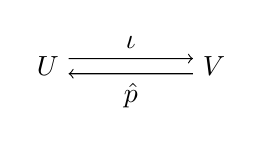
\begin{tikzpicture}[node distance = 6em, auto]
  \node (U) {$U$};
  \node (V) [right of = U] {$V$};
  \draw[->] (U.20) to node {$\iota$}(V.160);
  \draw[->] (V.200) to node {$\hat{p}$} (U.340);
 \end{tikzpicture}
\end{center}
where both maps are $G$-equivariant and $\hat{p} \iota = \id_U$. So the projection $\hat{p}$ splits and we obtain $V \cong U \oplus \ker \hat{p}$. Because $\hat{p}$ is $G$-equivariant $\ker \hat{p}$ is a subrepresentation of $V$. So $U$ has a complement which is again a representation.
\end{proof}

\begin{warn}
 The theorem is wrong in general if $\kchar k \mid |G|$. (An example will be on the exercise sheet.)
\end{warn}

\begin{expl}
 In general it is hard to compute a decomposition using Maschke’s theorem in practice!
 
 Let $G = S_3$. Let $V = kG$ be viewed as a representation of $G$ via the left multiplication, i.e.
 \[
  h.\left(\sum_{g \in G} a_g g\right) = \sum_{g \in G} a_g hg.
 \]
 Let $k = \C$, hence Maschke’s theorem holds. We want to find a decomposition of $kG$. Recall that $S_3 = \gen{s,t}$ where $s = (1 \; 2)$ and $t = (2 \; 3)$. We claim that
 \[
  kG = V_{\text{triv}} \oplus V_{\text{sgn}} \oplus V_1 \oplus V_2
 \]
 where
 \begin{align*}
  V_{\text{triv}} &:= \vspan\left(\sum_{g \in G} g \right) = \vspan(e+s+t+st+ts+sts), \\
  V_{\text{sgn}} &:= \vspan\left(e-s-t+st+ts-sts\right), \\
  V_1 &:= \vspan\left(e+s-ts, t+ts-st-sts\right) \text{ and} \\
  V_2 &:= \vspan\left(s+st-sts,e+t-s-st\right).
 \end{align*}
 Note that $G$ acts trivially on $V_{\text{triv}}$ and by multiplication with $-1$ on $V_{\text{sgn}}$ , hence $V_{\text{triv}}$ and $V_{\text{sgn}}$ are subrepresentations. One can also check that $V_1$ and $V_2$ are irreducible subrepresentations which are isomorphic.
\end{expl}


\begin{expl}
 Let $n \geq 2$ and $G = S_n$. Let $k$ be any field and let $S_n$ act on $k^n$ by setting
 \[
  g.e_i = e_{g(i)}
 \]
 where $e_1, \ldots, e_n$ denotes the standard basis of $k^n$. Extending this linearly we get a representation of $G$ on $k^n$, i.e.
 \[
  g.(a_1, \ldots, a_n) = \left(a_{g^{-1}(1)}, \ldots, a_{g^{-1}(n)}\right).
 \]
 We can then set $V = k^n$ and extend the $G$-action on $V$ to be a $G$-action on $\mc{P}(V)$ by setting $(g.f)(v) = f(g^{-1}.v)$ for all $f \in \mc{P}(V), v \in V$. We can then ask ourselves how to describe $\mc{P}(V)$.
\end{expl}


\begin{defi}
 Let $k$ be a group and $W$ any $k$-vector space. Then $g.w = w$ for all $g \in G, w \in W$ defines a representation $W$ of $G$. This is called the trivial representation. For each fixed dimension there is (up to isomorphism) one trivial representation. Therefore we usually say \emph{the} trivial representation of $G$ (of dimension $\dim W$).
\end{defi}


\begin{lem}
 Let $\{e_1, \ldots, e_n\}$ denote the standard basis von $k^n$. $G = S_n$ acts linearly on $k^n$ as in the previous example.
 \begin{enumerate}[a)]
  \item
  The vector subspaces
  \begin{gather*}
   U_1 := \vspan\left( \sum_{i=1}^n e_i\right)
  \shortintertext{and}
   U_2 := \left\{ (\lambda_1, \ldots, \lambda_n) \in k^n \,\middle|\, \sum_{i=1}^n \lambda_i = 0 \right\}
  \end{gather*}
  are subrepresentations.
  \item
  $U_1$ is the trivial $1$-dimensional subrepresentation and
  \[
   \begin{cases}
    U_1 = U_2 & \text{if } n = 2, \kchar k = 2,\\
    U_1 \ncong U_2 & \text{otherwise}.
   \end{cases}
  \]
  \item
  If $n = 2$ then $V$ is completely reducible if and only if $\kchar k \neq 2$.
 \end{enumerate}
\end{lem}
\begin{proof}
 \begin{enumerate}
  \item
  It is clear that $U_1$ and $U_2$ are vector subspaces. Since
  \[
   g.\left(\sum_{i=1}^n e_i\right)
   = \sum_{i=1}^n e_{g(i)}
   = \sum_{i=1}^n e_i
   \tag{$\ast$}
  \]
  we have $g.u \in U_1$ for all $g \in G, u \in U_1$, thus $U_1$ is a subrepresentation. Since
  \[
   g.(\lambda_1, \ldots, \lambda_n) = \left( \lambda_{g^{-1}(1)}, \ldots, \lambda_{g^{-1}(n)} \right)
  \]
  we have $g.u \in U_2$ for all $g \in G, u \in U_2$, thus $U_2$ is a subrepresentation.
  \item
  We have that $g.u = u$ for all $u \in U$ by ($\ast$).  If $n > 2$ then
  \[
   \dim U_1 = 1 \neq \dim U_2
  \]
  and thus $U_1 \ncong U_2$.
  
  If $n = 2$ and $S_2 = \{e,s\}$ then $s.(1,1) = (1,1)$ for the basis vector $(1,1)$ of $U_1$ and $s.(1,-1) = -(1,-1)$ for the basis vector $(1,-1)$ of $U_2$. So $U_2$ is not the trivial representation if $\kchar k \neq 2$, and thus $U_1 \ncong U_2$.  If $\kchar k = 2$ then $U_1$ and $U_2$ are both spanned by $(1,1)$ and thus $U_1 = U_2$.
  \item
  If $\kchar k \neq 2$ then $V$ is completely reducible by Maschke’s Theorem. If $\kchar k = 2$ then $U_1 = U_2$. This is the only one-dimensonal subrepresentation of $V$: If $U \subseteq V$ is a subrepresentation such that there exists $(\lambda, \mu) \in U$ with $\lambda \neq \mu$, then $(\mu, \lambda) \in U$ and thus $U = V$. Thus $V$ is indecomposible but reducible.
  \qedhere
 \end{enumerate}
\end{proof}


\begin{rem}
 In the case of $n = 2$ the representation $U_2$ is called the sign representation.
 %TODO: Sign-Darstellung besser erklären.
\end{rem}


\section{Symmetric Polynomials}


\begin{defi}
 Let $k$ be a field. $G := S_n$ acts linearly on $k[X_1, \ldots, X_n]$ by extending
 \[
  g.X^{\alpha_1} \cdots X_n^{\alpha_n} = X_{g(1)}^{\alpha_1} \cdots X_{g(n)}^{\alpha_n} \text{ for all } g \in G
 \]
 linearly. A polynomial $f \in k[X_1, \ldots, X_n]^{S_n}$ is called a symmetric polynomial (in $n$ variables).
\end{defi}


\begin{rem}
 For $k$ infinite we have an isomorphism of representations
 \[
  \Phi : k[X_1, \ldots, X_n] \to \mc{P}(k^n), X_i \mapsto \varphi_i,
 \]
 where $S_n$ acts on $\mc{P}(k^n)$ via
 \[
  (\sigma.f)(v) = f\left( \sigma^{-1}.v \right) \text{ for all } \sigma \in S_n, f \in \mc{P}(V), v \in k^n.
 \]
 We know that $\Phi$ is an isomorphism of $k$-vector spaces. It is $S_n$-equivariant, since for all $\sigma \in G, p = X_1^{\alpha_1} \cdots X_n^{\alpha_n} \in k[X_1, \ldots, X_n]$ and $v = (\lambda_1, \ldots, \lambda_n) \in k^n$
 \begin{align*}
  \Phi(g.p)(v)
  &= \Phi\left( X_{g(1)}^{\alpha_1} \cdots X_{g(n)}^{\alpha_n} \right)(v)
  = \lambda_{g(1)}^{\alpha_1} \cdots \lambda_{g(n)}^{\alpha_n} \\
  &= \Phi(p)( \lambda_{g(1)}, \ldots, \lambda_{g(n)} )
  = \Phi(p)\left( g^{-1}.(\lambda_1, \ldots, \lambda_n) \right) \\
  &= (g.\Phi(p))(\lambda_1, \ldots, \lambda_n).
 \end{align*}
\end{rem}


\begin{expl}
 In $k[X_1, X_2, X_3]$ we have the symmetric polynomials
 \begin{align*}
  p_2 &:= X_1^2 + X_2^2 + X_3^2, \\
  h_2 &:= X_1^2 + X_1 X_2 + X_1 X_3 + X_2^2 + X_2 X_3 + X_3^2, \\
  e_2 &:= X_1 X_2 + X_1 X_3 + X_2 X_3 \text{ and} \\
  m_{(4,4,2)} &:= X_1^4 X_2^2 X_3^2 + X_1^2 X_2^4 X_3^2 + X_1^2 X_2^2 X_3^4.
 \end{align*}
 More generally in $k[X_1, \ldots, X_n]$ we have the following symmmetric polynomials:
\end{expl}


\begin{defi}
 Fix $n \in \N$. The $r$-th power symmetric polynomial, also called the $r$-th power sum, is defined as
 \[
  p_r^{(n)} := X_1^r + \ldots + X_n^r,
 \]
 the $r$-th completely symmetric polynomial as
 \[
  h_r^{(n)} := \sum_{|\alpha|=r} X_1^{\alpha_1} \cdots X_n^{\alpha_n}.
 \]
 and the $r$-th elementary symmetric polynomial as
 \[
  e_r^{(n)} := \sum_{1 \leq i_1 < \ldots < i_r \leq n} X_{i_1} \cdots X_{i_r}.
 \]
 We also set $e_0^{(n)} := 1$ and $e_r^{(n)} = 0$ for $r > n$. If the number of variables in clear we also write $p_r$, $h_r$ and $e_r$.
\end{defi}

Another possible way of writing $e^{(n)}_r$ is
\[
 e^{(n)}_r = \sum_{\substack{I \subseteq \{1, \ldots, n\} \\ |I| = r}} \prod_{i \in I} X_i.
\]
From this we get that $e^{(n)}_0 = 1$ because the only subset of $\{1, \ldots, n\}$ which contains $0$ elements is the empty set and thus the sum consists only of the empty product. We also get that $e^{(n)}_r = 0$ for $r > n$ since $\{1, \ldots, n\}$ has no subsets which contain more than $n$ elements.

The elementary symmetric polynomials appear in very natural ways. If, for example, we have elements $a_1, \ldots, a_n \in k$ then we have
\begin{align*}
  &\, (t-a_1) \cdots (t-a_n) \\
 =&\, t^n - (a_1 + \ldots + a_n) t^{n-1} + \sum_{1 \leq i_1 < i_2 \leq n} a_{i_1} a_{i_2} t^{n-2} + \ldots + (-1)^n a_1 \cdots a_n \\ 
 =&\, t^n - e^{(n)}_1(a_1, \ldots, a_n) t^{n-1} + e^{(n)}_2(a_1, \ldots, a_n) t^{n-2} + \ldots + (-1)^n e^{(n)}_n(a_1, \ldots, a_n)
\end{align*}
in $k[t]$. We will formalize this observation in the following lemma.


\begin{lem}
 For all $n \in \N$ we have
 \[
  \prod_{i=1}^n (t-X_i) = t^n - e^{(n)}_1 t^{n-1} + e^{(n)}_2 t^{n-2} + \ldots + (-1)^n e^{(n)}_n
 \]
 in $k[X_1, \ldots, X_n][t]$.
\end{lem}
\begin{proof}
 For $n = 0$ the statement is clear. For $n \geq 1$ the coefficient of the left-hand side of $t^{n-r}$ is $e^{(n)}_0 = 1$ for $r = 0$ and
 \[
  \sum_{1 \leq i_1 < \ldots < i_r \leq n} (-X_{i_1}) \cdots (-X_{i_r}) = (-1)^r e^{(n)}_r.
 \]
 for $0 < r \leq n$.
\end{proof}


\begin{cor}
 For all $n \in \N$ we have
 \[
  p^{(n)}_n - e^{(n)}_1 p^{(n)}_{n-1} + e^{(n)}_2 p^{(n)}_{n-2} + \ldots + (-1)^n n e^{(n)}_n = 0.
 \]
\end{cor}
\begin{proof}
 For $n = 0$ the statement is clear. For $n > 0$ we have
 \[
  \prod_{i=1}^n (t-X_i) = t^n - e^{(n)}_1 t^{n-1} + e^{(n)}_2 t^{n-2} + \ldots + (-1)^n e^{(n)}_n
 \]
 and evaluating at $t = X_j$ gives
 \[
  X_j^n - e^{(n)}_1 X_j^{n-1} + e^{(n)}_2 X_j^{n-2} + \ldots + (-1)^n e^{(n)}_n = 0.
 \]
 By summing over all $1 \leq j \leq n$ we get
 \[
  p^{(n)}_n - e^{(n)}_1 p^{(n)}_{n-1} + e^{(n)}_2 p^{(n)}_{n-2} + \ldots + (-1)^n n e^{(n)}_n = 0.
 \]
\end{proof}


\begin{rem}[Newton’s identities]
 One can show that more generally
 \[
  p^{(n)}_m - e^{(n)}_1 p^{(n)}_{m-1} + \ldots + (-1)^{m-1} e^{(n)}_{m-1} p^{(n)}_1 + (-1)^m+ m e^{(n)}_m = 0.
 \]
 for all $m \geq 0$. For $m = n$ this gives us the previous corollary.
\end{rem}
\begin{proof}
 The proof of these identities is an exercise on the 4th exercise sheet. We will also give a proof later on.
\end{proof}


\begin{thrm}[Fundamental Theorem of symmetric functions]
 The symmetric polynomials $e^{(n)}_1, \ldots, e^{(n)}_n$ generate the $k$-algebra of symmetric functions $k[X_1, \ldots, X_n]^{S_n}$. Moreover they are algebraically independent. In other words
 \[
  k[X_1, \ldots, X_n]^{S_n} \cong k[X_1, \ldots, X_n] \text{ via } e^{(n)}_k \mapsto X_k.
 \]
\end{thrm}


\begin{lem}
 A polynomial $f \in k[X_1, \ldots, X_n]$ is symmetric if and only if its homogeneous parts are symmetric.
\end{lem}
\begin{proof}
 We have $k[X_1, \ldots, X_n] = \bigoplus_{d \geq 0} k[X_1, \ldots, X_n]_d$ as a graded $k$-algebra. We write $f = \sum_{d \geq 0} f_d$ where $f_d$ is the homogenous part of $f$ of degree $d$ and only finitely many $f_d$ are non-zero. We need to show that $f$ is symmetric if and only if $f_d$ is symmetric for all $d \geq 0$.
 
 Is is clear that $f$ is symmetric if all $f_d$ are symmetric. On the other hand we notice that the decomposition $k[X_1, \ldots, X_n] = \bigoplus_{d \geq 0} k[X_1, \ldots, X_n]$ into vector subspaces is also a decomposition into subrepresentations of $S_n$. If $f$ is symmetric we therefore have for all $\sigma \in S_n$
 \[
  f = \sum_{d \geq 0} f_d = \sigma.\left( \sum_{d \geq 0} f_d \right) = \sum_{d \geq 0} \sigma.f_d.
 \]
 Because the sum is direct and $\sigma.f_d \in k[X_1, \ldots, X_n]_d$ for all $d \geq 0$ we have $\sigma.f_d = f_d$ for all $d \geq 0$.
\end{proof}


Using this Lemma we can now easily prove the Fundamental Theorem. We will give two possible proofs. The first one is shorter and more intuitive while the second one was given in the lecture.


\begin{proof}[Proof of the Fundamental Theorem]
To makes our lifes easier we introduce an ordering on the monomials in $k[X_1, \ldots, X_n]$: We first order the monomials by their power of $X_1$ from lowest to highest. The monomials with the same power of $X_1$ are then ordered in the same way by their power of $X_2$, then those with the same power of $X_2$ by their power of $X_3$, and so on. In a more formal way: For monomials $X^\alpha = X_1^{\alpha_1} \cdots X_n^{\alpha_n}$ and $X^\beta = X_1^{\beta_1} \cdots X_n^{\beta_n}$ we have $X^\alpha > X^\beta$ if and only if there exists $1 \leq i \leq n$ such that $\alpha_1 = \beta_1, \alpha_2 = \beta_2, \ldots, \alpha_{i-1} = \beta_{i-1}$ and $\alpha_i > \beta_i$. This gives us a total order on the monomials in $k[X_1, \ldots, X_n]$.
 
 For a polynomial $p \in k[X_1, \ldots X_n]$ with $p \neq 0$ we define $\init p$ to be the highest monomial occuring in $p$, including its coefficient. One can easily check the following properties:
 \begin{enumerate}
  \item
   If $p$ is symmetrical and $\init p = c X_1^{\alpha_1} \cdots X_n^{\alpha_n}$ we have $\alpha_1 \geq \alpha_2 \geq \ldots \geq \alpha_n$.
  \item
   For $q \in k[X_1, \ldots, X_n], q \neq 0$ we have $\init (p \cdot q) = \init p \cdot \init q$.
  \item
   $\init e^{(n)}_k = X_1 \cdots X_k$ for all $1 \leq k \leq n$.
 \end{enumerate}
 We are now well-equipped to prove the Theorem. 
 
 We first show that $e^{(n)}_1, \ldots, e^{(n)}_n$ generate $k[X_1, \ldots, X_n]^{S_n}$ as a $k$-algebra. For this let $f \in k[X_1, \ldots, X_n]^{S_n}$ with $f \neq 0$. By the previous Lemma we may assume that $f$ is homogeneous of degree $d \geq 0$. For
 \[
  \init f = c X_1^{\alpha_1} \cdots X_n^{\alpha_n}
 \]
 we define
 \[
  p = c \left(e^{(n)}_1\right)^{\alpha_1 - \alpha_2} \cdots \left(e^{(n)}_{n-1}\right)^{\alpha_{n-1} - \alpha_n} \left(e^{(n)}_n\right)^{\alpha_n}.
 \]
 From the properties listed above it directly follows that that $p$ is well defined with $\init p = \init f$. Because $e^{(n)}_k$ is homogenous of degree $k$ it follows that $p$ is homogeneous of degree
 \begin{align*}
   &\,(\alpha_1-\alpha_2) + 2(\alpha_2-\alpha_3) + \ldots + (n-1)(\alpha_{n-1}-\alpha_n)+n\alpha_n \\
  =&\, \alpha_1 + \ldots + \alpha_n
  = d.
 \end{align*}
 (Because $f$ is homogenous we have $d = \deg f = \deg \init f = \alpha_1 + \ldots + \alpha_n$.) Combining these observations we find that $f-p$ is a homogeneous symmetric polynomial of degree $d$ with either $f-p = 0$ or at least $\init (f-p) < \init f$. Because there are only finitely many monomials of degree $d$ repeating this procedure must lead us to the zero polynomial in finitely many steps.
 
 To show that $e^{(n)}_1, \ldots, e^{(n)}_n$ are algebraically independent we need to show that the monomials in $e^{(n)}_1, \ldots, e^{(n)}_n$, i.e.
 \[
  \left(e^{(n)}\right)^\alpha = \left(e^{(n)}_1\right)^{\alpha_1} \cdots \left(e^{(n)}_n\right)^{\alpha_n} \text{ with } \alpha = (\alpha_1, \ldots, \alpha_n)
 \]
 are linearly independent. For this we notice that for $(\alpha_1, \ldots, \alpha_n) \neq (\beta_1, \ldots, \beta_n)$ we have
 \begin{align*}
      &\, \init \left(e^{(n)}_1\right)^{\alpha_1} \cdots \left(e^{(n)}_n\right)^{\alpha_n} \\
     =&\, X_1^{\alpha_1 + \ldots + \alpha_n} X_2^{\alpha_1 + \ldots + \alpha_{n-1}} \cdots X_n^{\alpha_n} \\
  \neq&\, X_1^{\beta_1 + \ldots + \beta_n} X_2^{\beta_1 + \ldots + \beta_{n-1}} \cdots X_n^{\beta_n} \\
     =&\, \init \left(e^{(n)}_1\right)^{\beta_1} \cdots \left(e^{(n)}_n\right)^{\beta_n}.
 \end{align*}
 Now suppose that
 \[
  0 = \lambda_1 \left(e^{(n)}\right)^{\alpha_1} + \ldots + \lambda_s \left(e^{(n)}\right)^{\alpha_s}
 \]
 with $s \geq 1$, $\alpha_i \neq \alpha_j$ for $i \neq j$ and $\lambda_i \neq 0$ for all $1 \leq i \leq s$. We can assume w.l.o.g. that 
 \[
  \init \left(e^{(n)}\right)^{\alpha_1} > \init \left(e^{(n)}\right)^{\alpha_2} > \ldots > \init \left(e^{(n)}\right)^{\alpha_s}.
 \]
 With this we directly find that the $\init \left(e^{(n)}\right)^{\alpha_1}$ only occures in $\left(e^{(n)}\right)^{\alpha_1}$ and thus $\lambda_1 = 0$, in contradiction to $\lambda_1 \neq 0$.
\end{proof}


\begin{proof}[Proof of the Fundamental Theorem (lecture)]
 Note that
 \begin{align*}
  e^{(n)}_1 &= X_1 + \ldots + X_n = e_1^{(n-1)} + X_n, \\
  e^{(n)}_2 &= \sum_{1 \leq i_1 < i_2 \leq n} X_{i_1} X_{i_2} = e_2^{(n-1)} + X_n e_1^{(n-1)}, \\
            &\vdots \tag{$\ast$}\\ 
  e^{(n)}_r &= e^{(n-1)}_r + X_n e^{(n-1)}_{r-1} \text{ for } 1 \leq r \leq n-1, \\
            &\vdots \\
  e^{(n)}_n &= X_1 \cdots X_{n-1} X_n = X_n e^{(n-1)}_{n-1}.
 \end{align*}
 \begin{claim}
  A polynomial $f \in k[X_1, \ldots, X_n]$ is symmetric if and only if $f$ can be written as a polyonmial in $e^{(n)}_1, \ldots, e^{(n)}_n$, i.e. we have
  \[
   k\left[e^{(n)}_1, \ldots, e^{(n)}_n\right] = k[X_1, \ldots, X_n]^{S_n}.
  \]
 \end{claim}
 \begin{proof}[Proof of claim]
  It is clear that $k\left[e^{(n)}_1, \ldots, e^{(n)}_n\right] \subseteq k[X_1, \ldots, X_n]$. We show the other inclusion by induction over $n$.
  
  For $n = 1$ the claim is clear. Let $n \geq 2$ and suppose that the claim holds for $n-1$. We show the claim for $n$ by induction over $\deg f$. For $\deg f = 0$ the claim is clear. Let $d \geq 1$ and suppose the claim holds for $0, \ldots, d-1$. By the previous Lemma we may assume that $f$ is homogenous of degree $d$. (The homogenous parts of lower degree are by induction hypothesis expressable as polynomials in $e^{(n)}_1, \ldots, e^{(n)}_n$.) Let
  \[
   q : k[X_1, \ldots, X_n] \to k[X_1, \ldots, X_n]/(X_n) \cong k[X_1, \ldots, X_{n-1}]
  \]
  be the evaluation at $X_n = 0$. By $(\ast)$ we have
  \begin{align*}
   q\left( e^{(n)}_r \right) &= e^{(n-1)}_r \text{ for all } 1 \leq r < n \text{ and}\\
   q\left( e^{(n)}_n \right) &= 0.
  \end{align*}
  We notice that $q(f) \in k[X_1, \ldots, X_{n-1}]$ is symmetric: Because $f$ is symmetric we have
  \[
   f = f(X_1, \ldots, X_n) = f(X_{\sigma(1)}, \ldots, X_{\sigma(n)})
  \]
  for every $\sigma \in S_n$. Thus we have
  \[
   f(X_1, \ldots, X_{n-1}, 0) = f(X_{\tau(1)}, \ldots, X_{\tau(n-1)}, 0).
  \]
  for every $\tau \in S_{n-1}$. Because $q(f) \in k[X_1, \ldots, X_{n-1}]$ is symmetric we can use the induction hypothesis (from the induction on $n$) to write
  \[
   q(f) = P\left(e^{(n-1)}_1, \ldots, e^{(n-1)}_{n-1}\right)
  \]
  for some polynomial $P \in k[X_1, \ldots, X_{n-1}]$. Consider the symmetric polynomial
  \[
   g := P\left(e^{(n)}_1, \ldots, e^{(n)}_{n-1}\right) \in k[X_1, \ldots, X_n].
  \]
  Because $q$ is a $k$-algebra homomorphism we have
  \begin{align*}
   q(g)
   &= q\left( P\left(e^{(n)}_1, \ldots, e^{(n)}_{n-1}\right) \right) \\
   &= P\left( q\left(e^{(n)}_1\right), \ldots, q\left(e^{(n)}_{n-1}\right) \right) \\
   &= P\left( e^{(n-1)}_1, \ldots, e^{(n-1)}_{n-1} \right) \\
   &= q(f)
  \end{align*}
  and therefore
  \[
   q(f-g) = 0.
  \]
  Because $\ker q = (X_n)$ this means that $X_n \mid (f-g)$. Because $f-g$ is symmetric (because $f$ and $g$ are symmetric) it follows that $X_i \mid (f-g)$ for all $1 \leq i \leq n$. Therefore $X_1 \cdots X_n \mid (f-g)$ and we can set
  \[
   h := \frac{f-g}{X_1 \cdots X_n} = \frac{f-g}{e^{(n)}_n}.
  \]
  (Here we use that $k[X_1, \ldots, X_n]$ is an unique factorization domain.) We have $\deg h < \deg f = d$, since $\deg g \leq \deg f$. [I have no idea why $\deg g \leq \deg f$.] By induction hypothesis (of the induction on $d$) we can write $h$ as a polynomial in $e^{(n)}_1, \ldots, e^{(n)}_n$ and therefore also $f-g = h e^{(n)}_n$. Since $g$ is a Polynomial in $e^{(n)}_1, \ldots, e^{(n)}_n$ so is $f$.
  % TODO: Warum ist deg(g) <= deg(f)? Wofür die Homogenität von f? %
 \end{proof}
  All that is left to show is that $e^{(n)}_1, \ldots, e^{(n)}_n$ are algebraically independent. We prove this by induction over $n$.
  
  For $n = 1$ this is clear, since $e^{(1)}_1 = X_1$. Now suppose $n \geq 2$ and that the elements $e^{(n-1)}_1, \ldots, e^{(n-1)}_{n-1}$ are algebraically independent. Suppose that
  \[
   F\left(e^{(n)}_1, \ldots, e^{(n)}_n\right) = 0
  \]
  for some polynomial $F \in k[X_1, \ldots, X_n]$ with $F \neq 0$ of minimal possible degree. Then
  \begin{align*}
   0
   &= q\left(F\left(e^{(n)}_1, \ldots, e^{(n)}_{n-1} ,e^{(n)}_n\right)\right) \\
   &= F\left( q\left(e^{(n)}_1\right), \ldots, q\left(e^{(n)}_{n-1}\right), q\left(e^{(n)}_n\right) \right) \\
   &= F\left( e^{n-1}_1, \ldots e^{(n-1)}_{n-1}, 0 \right).
  \end{align*}
  Using the induction hypothesis we find that $F(X_1, \ldots, X_{n-1}, 0) = 0$. Therefore $X_n \mid F$. This means that there exists some $\hat{F} \in k[X_1, \ldots, X_n]$ with $F = X_n \hat{F}$. In particular $\hat{F} \neq 0$. We have
  \[
   0
   = F\left(e^{(n)}_1, \ldots, e^{(n)}_n\right)
   = e^{(n)}_n \hat{F}\left(e^{(n)}_1, \ldots, e^{(n)}_n\right).
  \]
  Because $k[X_1, \ldots, X_n]$ is an integral domain and $e^{(n)}_n \neq 0$ it follows that
  \[
   \hat{F}\left(e^{(n)}_1, \ldots, e^{(n)}_n\right) = 0.
  \]
  Because $\hat{F} \neq 0$ and $\deg \hat{F} < \deg F$ this contradicts the assumption that $F$ is of lowest possible degree.
\end{proof}


\begin{rem}
 Each of the proofs gives us an algorithm how to express a symmetric polynomial in terms of $e^{(n)}_1, \ldots, e^{(n)}_n$.
\end{rem}


\begin{rem}
 The Fundamental Theorem also holds for $k = \Z$.
\end{rem}


To better understand the polynomials $e^{(n)}_k$, $h^{(n)}_k$ and $p^{(n)}_k$ and how they interact with each other it is helpful to have a look at the corresponding generating functions in $k[X_1, \ldots, X_n]\dblbrack{t}$, i.e.
\begin{align*}
 E(t) &:= \sum_{k \geq 0} e^{(n)}_k t^k, \\
 H(t) &:= \sum_{k \geq 0} h^{(n)}_k t^k \text{ and} \\
 P(t) &:= \sum_{k \geq 0} p^{(n)}_{k+1} t^k.
\end{align*}
(Notice that for $P(t)$ we shift the index by $1$.)


\begin{prop}
 We have the following equalities of power series:
 \begin{enumerate}[1)]
  \item
   $E(t) = \prod_{i=1}^n (1 + X_i t)$.
  \item
   $H(t) = \prod_{i=1}^n \frac{1}{1 - X_i t}$.
  \item
   $P(t) = \sum_{i=1}^n \frac{X_i}{1 - X_i t}$. More generally $\sum_{k \geq 0} p_{k+l} t^k = \sum_{i=1}^n \frac{X_i^l}{1 - X_i t}$ for all $l \geq 0$.
 \end{enumerate}
\end{prop}
\begin{proof}
 \begin{enumerate}[1)]
  \item
   The coefficient of $t^r$ on the right hand side of the equation is
   \[
    \sum_{\substack{I \subseteq \{1, \ldots, n\} \\ |I| = r}} \prod_{i \in I} X_i,
   \]
   which is precisely $e^{(n)}_r$.
  \item
   It is clear that $1-X_i t$ is invertible in $k[X_1, \ldots, X_n]\dblbrack{t}$. (For a commutative ring $R$ a power series $\sum_{i \in \N} a_i t^i \in R\dblbrack{t}$ is invertible if and only if $a_0 \in R^\times$.) For $1 \leq i \leq n$ let
   \[
    Q_i := \frac{1}{1-X_i t} \in k[X_1, \ldots, X_n] \dblbrack{t}.
   \]
   We then have
   \[
    \prod_{i=1}^n \frac{1}{1-X_i t} = Q_1 \cdots Q_n.
   \]
   By using the geometric series it is now easy to see that
   \[
    Q_i = 1 + X_i t + X_i^2 t^2 + X_i^3 t^3 + \ldots.
   \]
   With this we find that the coefficient of $t^r$ in $Q_1 \cdots Q_n$ is
   \[
    \sum_{|\alpha| = r} X_1^{\alpha_1} \cdots X_n^{\alpha_n},
   \]
   which is precisely $h^{(n)}_r$.
  \item
   We have
   \begin{align*}
     &\, \sum_{i=1}^n \frac{X_i^l}{1-X_i t}
    =    \sum_{i=1}^n X_i^l Q_i \\
    =&\, \sum_{i=1}^n (X_i^l + X_i^{l+1} t + X_i^{l+2} t^2 + X_i^{l+3} t^3 + \ldots) \\
    =&\, p^{(n)}_l + p^{(n)}_{l+1} t + p^{(n)}_{l+2} t^2 + p^{(n)}_{l+3} t^3 + \ldots
   \end{align*}\qedhere
 \end{enumerate}
\end{proof}


From this equalities we can now easily derive more equalities.


\begin{cor}
 For all $s \geq 1$ we have
 \[
  h^{(n)}_s - e^{(n)}_1 h^{(n)}_{s-1} + e^{(n)}_2 h^{(n)}_{s-2} + \ldots + (-1)^{s-1} e^{(n)}_{s-1} h^{(n)}_1 + (-1)^s e^{(n)}_s = 0
 \]
 as well as
 \[
  e^{(n)}_s - h^{(n)}_1 e^{(n)}_{s-1} + h^{(n)}_2 e^{(n)}_{s-2} + \ldots + (-1)^{s-1} h^{(n)}_{s-1} e^{(n)}_1 + (-1)^s h^{(n)}_s = 0.
 \]
\end{cor}
\begin{proof}
 From the previous proposition it follows that
 \[
  E(-t)H(t) = H(-t)E(t) = 1.
 \]
 The first sum is the $s$-th coefficient of $E(-t)H(t)$ and the second sum is the $s$-th coefficient of $H(-t)E(t)$. One equation can also be obtained from the other by multiplying with $(-1)^s$.
\end{proof}


\begin{cor}
 For all $r \geq 1$ we have
 \[
  r h^{(n)}_r = p^{(n)}_1 h^{(n)}_{r-1} + p^{(n)}_2 h^{(n)}_{r-2} + \ldots + p^{(n)}_{n-1} h^{(n)}_1 + p^{(n)}_n.
 \]
\end{cor}
\begin{proof}
 By $H'(t)$ we denote the formal derivative of $H$ with respect to $t$. On the one hand we have
 \[
  H'(t) = \sum_{k \geq 1} k h^{(n)}_k t^{k-1}.
 \]
 On the other hand we have
 \[
  H'(t) = \sum_{i=1}^n \frac{X_i}{(1-X_i t)^2} \prod_{j \neq i} \frac{1}{1 - X_j t}
  = \sum_{i=1}^n \frac{X_i}{1 - X_i t} \prod_{j=1}^n \frac{1}{1 - X_j t}
  = P(t) H(t).
 \]
 By comparing the $(r-1)$-th coefficient on both expressions we find that
 \[
  r h^{(n)}_r = \sum_{i=0}^{r-1} p^{(n)}_{1+i} h_{r-1-i} = \sum_{i=1}^r p^{(n)}_i h^{(n)}_{r-i}
 \]
 for all $r \geq 1$.
\end{proof}


In the same way we can derive Newton’s identities as another corollary.


\begin{proof}[Proof of Newton’s identities]
 We have
 \[
  E'(t) = \sum_{k \geq 1} k e^{(n)}_k t^{k-1}
 \]
 as well as
 \[
  E'(t)
  = \sum_{i=1}^n X_i \prod_{j \neq i} (1 + X_j t)
  = \sum_{i=1}^n \frac{X_i}{1 + X_i t} \prod_{j=1}^n (1 + X_j t)
  = P(-t)E(t).
 \]
 Comparing the $(r-1)$-th coefficient of both expressions gives us
 \[
  r e^{(n)}_r
  = \sum_{i=0}^{r-1} (-1)^i p^{(n)}_{1+i} e^{(n)}_{r-1-i}
  = \sum_{i=1}^r (-1)^{i+1} p^{(n)}_i e^{(n)}_{r-i}.
 \]
 for all $r \geq 1$ and thus
 \begin{align*}
  0
  &= \sum_{i=0}^r (-1)^{i+1} p^{(n)}_i e^{(n)}_{r-i} \\
  &= (-1)^{r+1} p^{(n)}_r + (-1)^r p^{(n)}_{r-1} e^{(n)}_1 + \ldots + p^{(n)}_1 e^{(n)}_{r-1} - r e^{(n)}_r.
 \end{align*}
 Multplying by $(-1)^{r+1}$ results in Newton’s identities as they were given before.
\end{proof}



Using the first corallary we can not only give recursive formals for expressing $h^{(n)}_1, \ldots, h^{(n)}_n$ as polynomials in $e^{(n)}_1, \ldots, e^{(n)}_n$ (which we knew was possible from the Fundamental theorem) but also formulas for expressing $e^{(n)}_1, \ldots, e^{(n)}_n$ in polynomials of $h^{(n)}_1, \ldots, h^{(n)}_n$. Thus we find that $k[X_1, \ldots, X_n]^{S_n}$ is also generated by $h^{(n)}_1, \ldots, h^{(n)}_n$. One natural question which comes with this observation is whether $h^{(n)}_1, \ldots, h^{(n)}_n$ are also algebraically independent, which the symmetry of the two equations in the first corollary seem to hint at. Using this symmetrie we get the following Lemma.


\begin{lem}
 There exists polynomials $F_1, \ldots, F_n \in k[X_1, \ldots, X_n]$ such that
 \[
  h^{(n)}_i = F_i\left(e^{(n)}_1, \ldots, e^{(n)}_n\right) \text{ and }
  e^{(n)}_i = F_i\left(h^{(n)}_1, \ldots, h^{(n)}_n\right)
 \]
 for all $1 \leq i \leq n$.
\end{lem}
\begin{proof}
 We construct $F_1, \ldots, F_n$ recursively. Since $e^{(n)}_1 = h^{(n)}_1$ we start with $F_1 = X_1$. If $F_1, \ldots, F_{k-1}$ are already constructed for $k \leq n$ we set
 \[
  F_k := X_1 F_{k-1} - X_2 F_{k-2} + \ldots + (-1)^k X_{k-1} F_1 + (-1)^{k+1} X_k.
 \]
 From the first of the previous corollaries and the induction hypothesis it follows that
 \begin{align*}
   &\, F_k\left(e^{(n)}_1, \ldots, e^{(n)}_n\right) \\
  =&\, e^{(n)}_1 F_{k-1}\left(e^{(n)}_1, \ldots, e^{(n)}_n\right) - e^{(n)}_2 F_{k-2}\left(e^{(n)}_1, \ldots, e^{(n)}_n\right) + \ldots + (-1)^{k+1} e^{(n)}_k \\
  =&\, e^{(n)}_1 h^{(n)}_{k-1} - e^{(n)}_2 h^{(n)}_{k-2} + \ldots + (-1)^k e^{(n)}_{k-1} h^{(n)}_1 + (-1)^{k+1} e^{(n)}_k \\
  =&\, h^{(n)}_k,
 \end{align*}
 and by switching $e^{(n)}_i$ and $h^{(n)}_i$ we also find that
 \[
  F_k\left(h^{(n)}_1, \ldots, h^{(n)}_n\right) = e^{(n)}_k.
 \]
\end{proof}


With the help of this Lemma we can now easily prove the following Theorem, which points out a deep connection between the elementary symmetric polynomials and completely homogenous symmetirc polynomials and how they are, in a certain way, dual to each other.


\begin{thrm}
There exists an unique homomorphism
\[
 \phi : k[X_1, \ldots, X_n]^{S_n} \to k[X_1, \ldots, X_n]^{S_n}
\]
of $k$-algebras with $\phi\left(e^{(n)}_i\right) = h^{(n)}_i$ for all $1 \leq i \leq n$. $\phi$ in an automorphism and involutive
\end{thrm}
\begin{proof}
 The existence and uniqueness of $\phi$ follow directly from the fact that $e^{(n)}_1, \ldots, e^{(n)}_n$ generate $k[X_1, \ldots, X_n]^{S_n}$ as a $k$-algebra and are algebraically independent. (This is basically the universal property of the polynomial ring.) Using the previous Lemma we find that for all $1 \leq i \leq n$
 \begin{align*}
  \phi\left(h^{(n)}_i\right)
  &= \phi\left(F_i\left(e^{(n)}_1, \ldots, e^{(n)}_n\right)\right) \\
  &= F_i\left(\phi\left(e^{(n)}_1\right), \ldots, \phi\left(e^{(n)}_n\right)\right) \\
  &= F_i\left(h^{(n)}_1, \ldots, h^{(n)}_n\right)
  = e^{(n)}_i
 \end{align*}
 and thus
 \[
  \phi^2\left(e^{(n)}_i\right) = \phi\left(h^{(n)}_i\right) = e^{(n)}_i.
 \]
 Since $\phi^2\left(e^{(n)}_i\right) = e^{(n)}_i$ for all $1 \leq i \leq n$ we find that $\phi^2 = \id_{k[X_1, \ldots, X_n]^{S_n}}$ by using the universal property of the polynomial ring once more.
\end{proof}


This Theorem shows that $h^{(n)}_1, \ldots, h^{(n)}_n$ generate $k[X_1, \ldots, X_n]^{S_n}$ as a $k$-algebra and are algebraically independent. As for the Fundamental Theorem this result also holds for $k = \Z$.


Since $e^{(n)}_1, \ldots, e^{(n)}_n$ and $h^{(n)}_1, \ldots, h^{(n)}_n$ are each algebraically independent and generate $k[X_1, \ldots, X_n]^{S_n}$ for arbitrary fields and also $k = \Z$, it seems natural to ask if this is also true for $p^{(n)}_1, \ldots, p^{(n)}_n$. The next theorem shows that this is true under additional assumptions.


\begin{thrm}
 Let $k$ be a field with either $\kchar k = 0$ or $\kchar k > n$. Then $p^{(n)}_1, \ldots, p^{(n)}_n$ generate $k[X_1, \ldots, X_n]^{S_n}$ and are algebraically independent.
\end{thrm}
\begin{proof}
 We first show that $p^{(n)}_1, \ldots, p^{(n)}_n$ generate $k[X_1, \ldots, X_n]^{S_n}$ as a $k$-algebra. For this it is enough to show that $e^{(n)}_1, \ldots, e^{(n)}_n$ can be expressed as polynomials in $p^{(n)}_1, \ldots, p^{(n)}_n$. That this is possible follows directly from Newton’s identities. (Here we need that $2, \ldots, n$ are invertible in $k$.)
 
 To show that $p^{(n)}_1, \ldots, p^{(n)}_n$ are algebraically independent we need to show that the monomials in $p^{(n)}_1, \ldots, p^{(n)}_n$, i.e.
 \[
  \left(p^{(n)}\right)^\alpha = \left(p^{(n)}_1\right)^{\alpha_1} \cdots \left(p^{(n)}_n\right)^{\alpha_n} \text{ with } \alpha = (\alpha_1, \ldots, \alpha_n)
 \]
 are linearly independent. For this is sufficies to show that the monomials in $p^{(n)}_1, \ldots, p^{(n)}_n$ of degree $\leq N$ form a $k$-basis of the symmetric polynomials of degree $\leq N$. We denote the number of (pairwise different) monomials in $p^{(n)}_1, \ldots, p^{(n)}_n$ by $P_N$ and this subspace by $V_N$. Because $p^{(n)}_1, \ldots, p^{(n)}_n$ generate $k[X_1, \ldots, X_n]^{S_n}$ as a $k$-algebra we already know that $V_N$ is generated as a vector subspace by the monomials in $p^{(n)}_1, \ldots, p^{(n)}_n$ of degree $\leq N$. Thus $\dim V_N \leq P_N$. Because $e^{(n)}_1, \ldots, e^{(n)}_n$ generate $k[X_1, \ldots, X_n]^{S_n}$ as a $k$-algebra and are algebraically independent we also know that the monomials in $e^{(n)}_1, \ldots, e^{(n)}_n$ of degree $\leq N$ form a $k$-basis of $V_N$. We denote the number of these monomials by $E_N$ and have $\dim V_N = E_N$. Since $P_N \leq E_N$ we also have $P_N \leq \dim V_N$. (That $P_N \leq E_N$ follows from the fact that for each monomial in $p^{(n)}_1, \ldots, p^{(n)}_n$ we have a corresponding monomial in $e^{(n)}_1, \ldots, e^{(n)}_n$ of the same degree, i.e. we have a surjective map
\begin{align*}
    &\, \{\text{monomials in $e^{(n)}_1, \ldots, e^{(n)}_n$ of degree $\leq N$}\} \\
    &\, \to \{\text{monomials in $p^{(n)}_1, \ldots, p^{(n)}_n$ of degree $\leq N$}\}, \\
    &\, \left(e^{(n)}\right)^\alpha \mapsto \left(p^{(n)}\right)^\alpha,
\end{align*}
where we use that the monomials in $e^{(n)}_1, \ldots, e^{(n)}_n$ are pairwise different.)
Therefore we have $P_N = \dim V_N$, so the monomials in $p^{(n)}_1, \ldots, p^{(n)}_n$ of degree $\leq N$ are a $k$-basis of $V_N$.
\end{proof}


It is important to notice that the theorem does not hold for $k = \Z$! This is easy to see: In $\Q[X_1, X_2]^{S_2}$ we have
\[
 e^{(2)}_2 = \frac{1}{2}\left(p^{(2)}_1\right)^2 - \frac{1}{2} p^{(2)}_2.
\]
If $\Z[X_1, X_2]^{S_2}$ was generated by $p^{(n)}_1, p^{(n)}_2$ a polynomial $F \in \Z[X_1, X_2]$ with $e^{(2)}_2 = F\left(e^{(2)}_1, e^{(2)}_2\right)$ would exist. But this would contradict the algebraically independency of $p^{(2)}_1, p^{(2)}_2$ in $\Q[X_1, X_2]^{S_2}$ as $F(X_1, X_2) \neq \frac{1}{2} X_1^2 - \frac{1}{2} X_2$.


Using the same argumentation we find that for a symmetric polynomial $f \in \Q[X_1, \ldots, X_n]^{S_n}$ with integer coefficients and $F,G \in \Q[X_1, \ldots, X_n]^{S_n}$ with
\[
 f = F\left( e^{(n)}_1, \ldots, e^{(n)}_n \right) = G\left( h^{(n)}_1, \ldots, h^{(n)}_n\right)
\]
both $F$ and $G$ must have integer coefficients.


\begin{expl}
 Another example of formal power series are Hilbert series. Given a graded $k$-algebra $A = \bigoplus_{d \geq 0} A_d$ ($A_d = 0$ for $d < 0$) with $\dim_k A_d < \infty$ for all $d$ the corresponding Hilbert series is defined as
 \[
  P_A(t) := \sum_{d \geq 0} \left( \dim_k A_d \right) t^d \in k\dblbrack{t}.
 \]
 If $\dim_k A < \infty$ we have $P_A(t) \in k[t] \subseteq k\dblbrack{t}$.
 
 If $A = \bigoplus_{d \geq 0} A_d$ and $B = \bigoplus_{d \geq 0} B_d$ are graded $k$-algebras then $A \otimes_k B$ is a $k$-algebra via
 \[
  (a_1 \otimes b_1) (a_2 \otimes b_2) = (a_1 a_2) \otimes (b_1 b_2)
 \]
 and a graded $k$-algebra $A \otimes B = \bigoplus_{d \geq 0} (A \otimes B)_d$ by setting
 \[
  (A \otimes B)_d = \bigoplus_{i=0}^d (A_i \otimes B_{d-i}).
 \]
 We than have
 \[
  \dim_k (A \otimes B)_d = \sum_{i=0}^d \dim_k (A_i \otimes B_{d-i}) = \sum_{i=0}^d (\dim_k A_i) (\dim_k B_{d-i})
 \]
 for all $d \geq 0$ and thus
 \[
  P_{A \otimes B}(t) = P_A(t) P_B(t).
 \]
\end{expl}



\begin{defi}
 $\lambda = (\lambda_1, \ldots, \lambda_s) \in \N^s$ is a partition of $|\lambda| := \sum_{i=1}^s \lambda_i$ if
 \[
  \lambda_1 \geq \lambda_2 \geq \ldots \geq \lambda_s \geq 0.
 \]
 The $\lambda_i$ are the parts of $\lambda$ and $l(\lambda) := s$ is the length of  $\lambda$.
 
 An infinite partition is a sequence $\lambda_1, \lambda_2, \ldots \in \N$ with $\lambda_i = 0$ for all $i \geq s$ for some $s$ such that $(\lambda_1, \ldots, \lambda_s)$ is a partition. For a partition $(\lambda_1, \ldots, \lambda_s) \in \N^s$ the infinite partition associated to $\lambda$ is defined as
 \[
  \hat{\lambda}_i :=
  \begin{cases}
   \lambda_i & \text{for } 1 \leq i \leq l(\lambda) \\
           0 & \text{otherwise}.
  \end{cases}
 \]
 
 The transposed partition of a partition $\lambda$ is defined as
 \[
  \lambda'_i := |\{j \mid \lambda_j \geq i\}|.
 \]
\end{defi}

Partitions are often displayed in terms of Young diagrams. The Young diagram corresponding to a partition $\lambda$ is an array of boxes, left adjusted, such that the $i$-th row consists of $\lambda_i$ boxes.


\begin{expl}
 $\lambda = (4,2,2)$ is a partition of $8$ and $\lambda' = (3,3,1,1)$ is the transposed partion. The Young diagram corresponding to $\lambda'$ is the `transposition' of the Young diagram corresponding to $\lambda$. (See figure \ref{fig: Young diagram example}.)
 \begin{figure}
  \centering
  \ydiagram{4,2,2}
  \qquad
  \ydiagram{3,3,1,1}
  \caption{The Young diagrams corresponding to $\lambda$ (left) and to $\lambda'$ (right).}
  \label{fig: Young diagram example}
 \end{figure}
\end{expl}


\begin{defi}
 For $n \in \N$ we write
 \[
  \Par(n) := \{\text{partitions of $n$}\}
 \]
 and we set
 \[
  \Par := \bigcup_{n \in \N} \Par(n).
 \]
\end{defi}
 

\begin{defi}
 Let $\lambda$ and $\mu$ be partitions. We say that $\lambda \geq \mu$ if $|\lambda| = |\mu|$ and $\sum_{i=1}^r \hat{\lambda}_i \geq \sum_{i=1}^r \hat{\mu}_i$ for all $r$.
\end{defi}


\begin{expls}
 The following is a simple example of partitions of $6$.
 \[
  \ydiagram{6} > \ydiagram{4,2} > \ydiagram{3,3} > \ydiagram{3,2,1} > \ydiagram{1,1,1,1,1,1}
 \]
 The partitions
 \[
  \ydiagram{2,2} \quad \text{and} \quad \ydiagram{1,1}
 \]
 are not comparable (because $4 \neq 2$ in $\N$). The partitions
 \[
  \ydiagram{4,2,1,1,1} \quad \text{and} \quad \ydiagram{3,3,2,1}
 \]
 are also not comparable. (Because $4+2+1 = 7 < 8 = 3+3+2$ in $\N$.)
\end{expls}
%TODO: Bessere Erklärung der partiellen Ordnung hinzufügen.

\begin{lem}
 $\geq$ defines a partial ordering on $\Par$.
\end{lem}
\begin{proof}
 It is clear that $\geq$ is reflexive.
 
 If $\lambda$ and $\mu$ are partitions with $\lambda \geq \mu$ and $\lambda \leq \mu$ then $\lambda = \mu$: Because $\lambda \geq \mu$ we have $\lambda_1 \geq \mu_1$ and because $\lambda \leq \mu$ we have $\lambda_1 \leq \mu_1$. Thus we have $\lambda_1 = \mu_1$. In the same way we find that $\lambda_1 + \lambda_2 = \mu_1 + \mu_2$, and from $\lambda_1 = \mu_1$ we get that $\lambda_2 = \mu_2$. Because $|\lambda| = |\mu|$ we find inductively that $l(\lambda) = l(\mu)$ and $\lambda_i = \mu_i$ for all $1 \leq i \leq l(\lambda)$.
 
 If $\lambda, \mu$ and $\sigma$ are partitions with $\lambda \geq \mu$ and $\mu \geq \sigma$ then $\lambda \geq \sigma$: Because $\lambda \geq \mu$ we have $|\lambda| = |\mu|$ and because $\mu \geq \sigma$ we have $|\mu| = |\sigma|$. Thus we have $|\lambda| = |\sigma|$. For all $r \geq 1$ we have
 \[
  \sum_{i=1}^r \lambda_i \geq \sum_{i=1}^r \mu_i
  \text{ and }
  \sum_{i=1}^r \mu_i \geq \sum_{i=1}^r \sigma_i
 \]
 because $\lambda \geq \mu$ and $\mu \geq \sigma$, and therefore
 \[
  \sum_{i=1}^r \lambda_i \geq \sum_{i=1}^r \sigma_i.
 \]
\end{proof}


\begin{defi}
 Let $\lambda = (\lambda_1, \ldots, \lambda_r)$ be a partition. We define the elementary symmetric polynomial
 \[
  e^{(n)}_\lambda := e^{(n)}_{\lambda_1} \cdots e^{(n)}_{\lambda_r},
 \]
 the complete symmetric polynomial
 \[
  h^{(n)}_\lambda := h^{(n)}_{\lambda_1} \cdots h^{(n)}_{\lambda_r},
 \]
 the power symmetric polynomial
 \[
  p^{(n)}_\lambda := p^{(n)}_{\lambda_1} \cdots p^{(n)}_{\lambda_r}
 \]
 and the monomial symmetric polynomials
 \[
  m_\lambda := X_1^{\lambda_1} \cdots X_r^{\lambda_r} + \text{ all distinct permutations of this monomial}.
 \]
\end{defi}


One can also define $m_\lambda$ in a formal way: Instead of adding up all distinct permutations of the monomial $X_1^{\lambda_1} \cdots X_r^{\lambda_r}$ we can also take all distinct permutations of the tupel $\lambda$ and add up the corresponding monomials. To formalize this we let $S_r$ act on $\N^r$ by permuting the entries, i.e.
\[
 \pi.(a_1, \ldots, a_r) = \left( a_{\pi^{-1}(1)}, \ldots, a_{\pi^{-1}(r)} \right)
\]
for all $\pi \in S_r$ and $(a_1, \ldots, a_r) \in \N^r$. The set of all distinct permutations of $\lambda$ is precisely the orbit of $\lambda$ under this action. As we know from basic group theory we have an isomorphism of $G$-sets
\[
 S_r / U \to S_r \lambda, [\pi] \mapsto \pi.\lambda
\]
where $U$ is the stabilizer group of $\lambda$ and $S_r \lambda$ is the orbit of $\lambda$. (Note that $U$ is not necessarily a normal subgroup in $S_r$ and $S_r/U$ is only the set of left cosets.) Thus we can write
\[
 m_\lambda
 = \sum_{[\pi] \in S_r/U} X_1^{\lambda_{\pi^{-1}(1)}} \cdots X_r^{\lambda_{\pi^{-1}(r)}}
 = \sum_{[\pi] \in S_r/U} X_{\pi(1)}^{\lambda_1} \cdots X_{\pi(r)}^{\lambda_r}.
\]
Also notice that
\[
 U \cong S_{\nu_0} \times \cdots \times S_{\nu_m}
\]
where
\[
 \nu_n := \left|\left\{ 1 \leq i \leq r \mid \lambda_i = n \right\}\right|
\]
and $m := \max_{i=1,\ldots,r} \lambda_i$.


\begin{expl}[]
 [Here should be a part about Schur polynomials. However, some of the statements are unclear or wrong.]
 % TODO: Definition der Schubert Polynome liefern.
\end{expl}


\begin{lem}
 The set of monomial symmetric polynomials
 \[
  \{m_\lambda \mid \lambda \in \Par, l(\lambda) = n\}
 \]
 forms a $k$-basis of $k[X_1, \ldots, X_n]^{S_n}$ (as a $k$-vector space). More precisely
 \[
  \{m_\lambda \mid \lambda \in \Par, l(\lambda) = n, |\lambda|=d \}
 \]
 forms a $k$-basis of $k[X_1, \ldots, X_n]^{S_n}_d$.
\end{lem}
\begin{proof}
 Is is clear that
 \[
  \vspan_k \{m_\lambda \mid \lambda \in \Par, l(\lambda) = n, |\lambda|=d \} \subseteq k[X_1, \ldots, X_n]^{S_n}_d.
 \]
 On the other side let $f \in k[X_1, \ldots, X_n]^{S_n}_d$. By induction on the number of monomials of which $f$ consists we show that
 \[
  f \in \vspan_k \{m_\lambda \mid \lambda \in \Par, l(\lambda) = n, |\lambda|=d\}.
 \]
 For $f = 0$ this is clear. Suppose that $f \neq 0$ and that the statement is true for every polynomial in $k[X_1, \ldots, X_n]^{S_n}_d$ which consists of fewer monomials than $f$. Because $\{X^\alpha \mid \alpha \in \N^n, |\alpha|=d \}$ is a $k$-basis of $k[X_1, \ldots, X_n]_d$ we can write
 \[
  f = \sum_{\substack{\alpha \in \N^n \\ |\alpha|=d}} c_\alpha X^\alpha.
 \]
 with unique $c_\alpha \in k$ such that $c_\alpha \neq 0$ for only finitely many $\alpha$. Because $f$ is symmetric we find that
 \[
  c_\alpha = c_{\pi.\alpha} \text{ for all } \alpha \in \N^n, \pi \in S_n
 \]
 (where the action of $S_n$ on $\N^n$ is defined as above). Let $X^\beta$ be a monomial of $f$. Because $f \in k[X_1, \ldots, X_n]^{S_n}_d$ we have $X^\beta \in k[X_1, \ldots, X_n]_d$ and thus $c_\beta m_\beta \in k[X_1, \ldots, X_n]^{S_n}_d$. Because $c_\beta \neq 0$ and $c_\beta = c_{\pi.\beta}$ for every $\pi \in S_n$ we find that $f-c_{\beta}m_\beta$ consists of fewer monomials than $f$. Because $f-c_{\beta}m_\beta$ is symmetric we find by induction hypothesis that
 \[
  f - c_{\beta}m_\beta \in \vspan_k \{m_\lambda \mid \lambda \in \Par, l(\lambda) = n, |\lambda|=d\}.
 \]
 The statement for $f$ follows directly.
 
 To show that
 \[
  \{m_\lambda \mid \lambda \in \Par, l(\lambda) = n\}
 \]
 is linear independent we notice that for $\lambda, \mu \in \Par$ with $\lambda \neq \mu$ the polynomials $m_\lambda$ and $m_\mu$ have no monomials in common. Because
 \[
  \{X^\alpha \mid \alpha \in \N^n\}
 \]
 is linear independent it then follows that
 \[
  \{m_\lambda \mid \lambda \in \Par, l(\lambda) = n\}
 \]
 is linear independent.
\end{proof}


\begin{defi}
 Let $\lambda, \mu \in \Par$. We define the partition $\lambda+\mu$ of length $l(\lambda+\mu) = \max\{ l(\lambda), l(\mu) \}$ as
 \[
  (\lambda+\mu)_i =
  \begin{cases}
   \lambda_i + \mu_i & \text{if } i \leq l(\lambda),l(\mu), \\
   \lambda_i         & \text{if } i \leq l(\lambda), i > l(\mu), \\
   \mu_i             & \text{if } i \leq l(\mu), i > l(\lambda).
  \end{cases}
 \]
 So $\lambda+\mu$ is the partition of minimal length with
 \[
  \hat{\lambda}_i + \hat{\mu}_i = \widehat{\lambda+\mu}_i \text{ for all } i \geq 0.
 \]
\end{defi}


\begin{expl}
 For $\lambda = (4,4,2,2)$ and $\mu = (3,2,1)$ we have $\lambda+\mu = (7,6,3,2)$. The addition of two partitions can also easily be visualized with Young diagrams, see figure \ref{fig: addition partition young diagrams}.
 \begin{figure}\centering
  \[
   \ydiagram[*(gray)]{4,4,2,2} + \ydiagram[*(light-gray)]{3,2,1}
   = \ydiagram[*(light-gray)] {4+3,4+2,2+1} *[*(gray)]{7,6,3,2}
  \]
  \caption{Addition of partitions in term of Young diagrams.}
  \label{fig: addition partition young diagrams}
 \end{figure}
\end{expl}


\begin{lem}
 Let $\lambda, \mu \in \Par$. Then
 \[
  m_{\lambda} m_{\mu} = m_{\lambda + \mu} + \sum_{\nu < \lambda + \mu} a^\nu_{\lambda,\mu} m_\nu
 \]
 for suitable $a^\nu_{\lambda,\mu} \in k$. (This also holds for $k = \Z$.)
\end{lem}
\begin{proof}
 This is an exercise on the 4th exercise sheet.
\end{proof}


We know from the Fundamental Theorem that $e^{(n)}_1, \ldots, e^{(n)}_n$ generate the $k$-algebra of symmetric polynomials $k[X_1, \ldots, X_n]^{S_n}$ and are algebraically independent. This is equivalent to saying that the monomials in $e^{(n)}_1, \ldots, e^{(n)}_n$, i.e.
\[
 \left( e^{(n)} \right)^\alpha = \left(e^{(n)}_1\right)^{\alpha_1} \cdots \left(e^{(n)}_n\right)^{\alpha_n} \text{ with } \alpha = (\alpha_1, \ldots, \alpha_n)
\]
form a $k$-basis of $k[X_1, \ldots, X_n]^{S_n}$. We can also describe these polynomials in term of partitions.


\begin{prop}
 The monomials in $e^{(n)}_1, \ldots, e^{(n)}_n$ are precisely the polynomials $e^{(n)}_\lambda$ with $\lambda \in \Par$ such that $\lambda_1 \leq n$ and $\lambda_{l(\lambda)} \neq 0$.
\end{prop}
\begin{proof}
 On the one side the monomial $e_1^{\alpha_1} \cdots e_n^{\alpha_n}$ is the same as $e_\lambda$ for the partition
 \[
  \lambda = (\underbrace{n, \ldots, n}_{\alpha_n}, \underbrace{n-1, \ldots, n-1}_{\alpha_{n-1}}, \ldots, \underbrace{1, \ldots, 1}_{\alpha_1}).
 \]
 On the other side the polynomial $e_\lambda$ equals the monomial $e_1^{\nu_1(\lambda)} \cdots e_n^{\nu_n(\lambda)}$ for the exponents
 \[
  \nu_j(\lambda) = |\{1 \leq i \leq l(\lambda) \mid \lambda_i = j\}|.
 \]
 
 Notice that for $\lambda \neq \mu$ there exists some $1 \leq j \leq n$ with $\nu_j(\lambda) \neq \nu_j(\mu)$ (here we use that $1 \leq \lambda_i \leq n$ for all $1 \leq i \leq l(\lambda)$ and the same for $\mu$) and therefore
 \[
  e_1^{\nu_1(\lambda)} \cdots e_n^{\nu_n(\lambda)} \neq e_1^{\nu_1(\mu)} \cdots e_n^{\nu_n(\mu)}
 \]
 because the monomials in $e_1, \ldots, e_n$ are linearly independent.
\end{proof}


\begin{cor}
 The set
 \[
  B := \left\{ e^{(n)}_\lambda \,\middle|\, \lambda \in \Par, \lambda_1 \leq n, \lambda_{l(\lambda)} \neq 0 \right\}
 \]
 forms a $k$-basis of $k[X_1, \ldots, X_n]^{S_n}$ and the $e^{(n)}_\lambda$ are pairwise different. More precisely
 \[
  B_d := \left\{ e^{(n)}_\lambda \,\middle|\, \lambda \in \Par, \lambda_1 \leq n, \lambda_{l(\lambda)} \neq 0, |\lambda| = d \right\}
 \]
 forms a $k$-basis of $k[X_1, \ldots, X_n]^{S_n}_d$ for all $d \geq 0$.
\end{cor}


\begin{rem}
 Since $h^{(n)}_1, \ldots, h^{(n)}_n$ generate $k[X_1, \ldots, X_n]^{S_n}$ as a $k$-algebra and are algebraically independent we can show the same statements for the polynomials $h^{(n)}_\lambda$ with $\lambda \in \Par$ such that $\lambda_1 \leq n$ and $\lambda_{l(\lambda)} \neq 0$.
 
 In the case that $k$ is a field with $\kchar k = 0$ or $\kchar k > n$ we can show the same for the polynomials $p^{(n)}_\lambda$ with $\lambda \in \Par$ such that $\lambda_1 \leq n$ and $\lambda_{l(\lambda)} \neq 0$.
\end{rem}


% TODO: Basis aus Schurpolynomen hinzufügen.


\section{Polynomial maps.}


From here on let $k$ be an infinite field.


\begin{defi}
 Let $V$ and $W$ be finite dimensional $k$-vector spaces. A map $f : W \to V$ is called a polynomial map if, given a basis $(v_1, \ldots, v_n)$ of $V$, the coordinate functions of $f$ are polynomial, i.e. there exist $f_1, \ldots, f_n \in \mc{P}(W)$ with
 \[
  f(w) = \sum_{i=1}^n f_i(w) v_i
 \]
 for all $w \in W$.
\end{defi}


\begin{rem}
 One can show (as for $\mc{P}(W)$) that the definition doesn’t depend on the chosen basis of $V$.
\end{rem}


\begin{rem}
 If $V = k$ then $f : W \to k$ is a polynomial map if and only if $f \in \mc{P}(W)$.
\end{rem}


\begin{expl}
 Let $W$ be a finite dimensional $k$-vector space. Then
 \[
  f : W \to W^{\otimes r}, w \mapsto w \otimes \ldots \otimes w.
 \]
 is a polynomial map. To see this choose a basis $w_1, \ldots, w_n$ of $W$. Then the elements
 \[
  w_{\underline{i}} = w_{i_1} \otimes \ldots \otimes w_{i_r} \text{ with } \underline{i} = (i_1, \ldots, i_r) \in \{1, \ldots, n\}^r
 \]
 form a basis of $W^{\otimes r}$. For $w \in W$ with $w = \sum_{i=1}^r \lambda_i w_i$ we have
 \[
  f(w)
  = w \otimes \ldots \otimes w
  = \left( \sum_{i=1}^r \lambda_i w_i \right) \otimes \ldots \otimes \left( \sum_{i=1}^r \lambda_i w_i \right)
  = \sum_{\underline{i}} \lambda_{i_1} \cdots \lambda_{i_r} w_{\underline{i}}.
 \]
 For the polynomials
 \[
  p_{\underline{i}} = X_{i_1} \cdots X_{i_r}
 \]
 and polynomial maps $f_{\underline{i}} : W \to k$ with
 \[
  f_{\underline{i}}\left(\sum_{i=1}^r \lambda_i w_i\right) = p_{\underline{i}}(\lambda_1, \ldots, \lambda_r)
 \]
 we thus have
 \[
  f(w) = \sum_{\underline{i}} f_{\underline{i}}(w) w_{\underline{i}}.
 \]
\end{expl}


It is easy to see that the class of finite-dimensional $k$-vector spaces together with the polynomial maps between them form a category. We will denote this category by $\cpol_k$  Also notice that every linear map between finite-dimensional $k$-vector spaces is a polynomial map. Therefore $\cvect_k$ is a subcategory of $\cpol_k$.


\begin{lem}
 For a finite-dimensional $k$-vector space $V$ the map $\id_V : V \to V$ is a polynomial map. If $U$ and $W$ are finite-dimensonial vector spaces and $f : W \to V$ and $g : V \to U$ are polynomial maps then $gf : W \to U$ is also a polynomial map.
\end{lem}
\begin{proof}
 The first statement is clear. To show the second let $v_1, \ldots, v_r$ be a basis of $V$, $w_1, \ldots, w_s$ be a basis of $W$ and $u_1, \ldots, u_t$ be a basis of $U$. Because $f$ is a polynomial map we can find polynomials $P_1, \ldots, P_s \in k[X_1, \ldots, X_r]$ such that
 \[
  f\left(\sum_{i=1}^r \lambda_i v_i\right) = \sum_{j=1}^s F_j(\lambda_1, \ldots, \lambda_r) w_j
 \]
 and because $g$ is a polynomial map we can find polynomials $Q_1, \ldots, Q_t \in k[X_1, \ldots, X_s]$ such that
 \[
  g\left(\sum_{j=1}^s \mu_j w_j\right) = \sum_{k=1}^t G_k(\mu_1, \ldots, \mu_s) u_k.
 \]
 Combining this we find that
 \begin{align*}
  gf\left(\sum_{i=1}^r \lambda_i v_i\right)
  &= g\left(\sum_{j=1}^s F_j(\lambda_1, \ldots, \lambda_r) w_j\right) \\
  &= \sum_{k=1}^t Q_k(F_1(\lambda_1, \ldots, \lambda_r), \ldots, F_s(\lambda_1, \ldots, \lambda_r)) w_k \\
  &= \sum_{k=1}^t R_k(\lambda_1, \ldots, \lambda_r) w_k
 \end{align*}
 for the polynomials
 \[
  R_k := Q_k(F_1(X_1, \ldots, X_r), \ldots, F_s(X_1, \ldots, X_r)) \in k[X_1, \ldots X_r].
 \]
\end{proof}


















